\tikzstyle{tag} = [minimum height=1.5em, text width=5em, anchor=west]
\tikzstyle{tag2} = [minimum height=1.5em, text width=5em, anchor=east]
\tikzstyle{letter} = [draw, thin, fill=blue!50, minimum height=1.5em, minimum width=1.5em]
\tikzstyle{module} = [rectangle, draw, thin, fill=green!50, minimum height=1.5em]
\tikzstyle{module-1} = [module, minimum width=1.5em]
\tikzstyle{module-2} = [module, minimum width=7.5em]
\tikzstyle{module-3} = [module, minimum width=25.5em]

    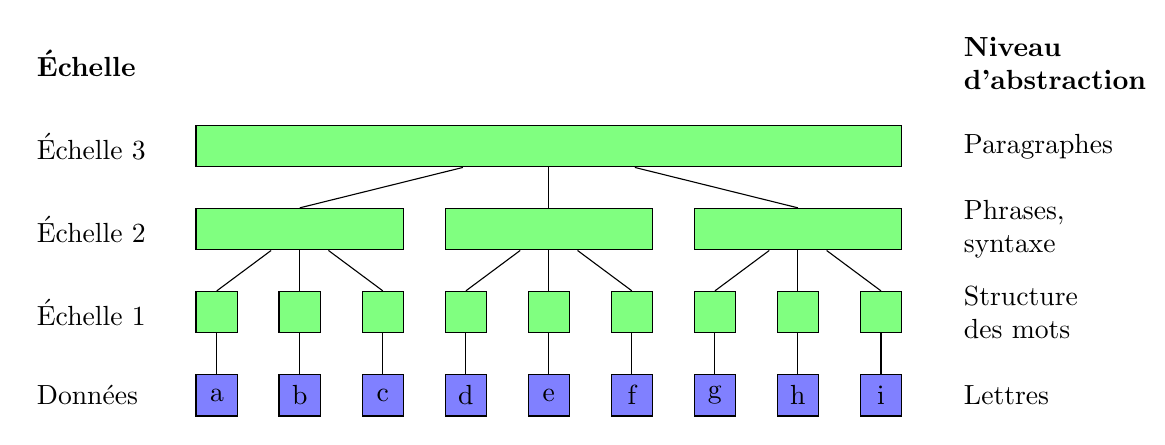
\begin{tikzpicture}[node distance=3em]
      \node[letter] (a) {a};
      \node[letter, right of=a] (b) {b};
      \node[letter, right of=b] (c) {c};
      \node[letter, right of=c] (d) {d};
      \node[letter, right of=d] (e) {e};
      \node[letter, right of=e] (f) {f};
      \node[letter, right of=f] (g) {g};
      \node[letter, right of=g] (h) {h};
      \node[letter, right of=h] (i) {i};
      
      \node[tag, right of=i, node distance=5.5em] (letters) {Lettres};
      \node[tag2, left of=a, node distance=4em] (e1) {Donn\'{e}es};
      
      \node[module-1, above of=a] (m-a) {};
      \node[module-1, above of=b] (m-b) {};
      \node[module-1, above of=c] (m-c) {};
      \node[module-1, above of=d] (m-d) {};
      \node[module-1, above of=e] (m-e) {};
      \node[module-1, above of=f] (m-f) {};
      \node[module-1, above of=g] (m-g) {};
      \node[module-1, above of=h] (m-h) {};
      \node[module-1, above of=i] (m-i) {};
      
      \node[tag, right of=m-i, node distance=5.5em] (word) {Structure des mots};
      \node[tag2, left of=m-a, node distance=4em] (e1) {\'{E}chelle 1};
      
      \node[module-2, above of=m-b] (m-abc) {};
      \node[module-2, above of=m-e] (m-def) {};
      \node[module-2, above of=m-h] (m-ghi) {};
      
      \node[tag, right of=m-ghi, node distance=8.5em] (sentence) {Phrases, syntaxe};
      \node[tag2, left of=m-abc, node distance=7em] (e2) {\'{E}chelle 2};
      
      \node[module-3, above of=m-def] (m-) {};
      
      \node[tag, right of=m-, node distance=17.5em] (paragraph) {Paragraphes};
      \node[tag2, left of=m-, node distance=16em] (e3) {\'{E}chelle 3};
      \node[tag, above of=paragraph, text width=5.9em, xshift=.45em, font=\bfseries] {Niveau d'abstraction};
      \node[tag2, above of=e3, font=\bfseries] {\'{E}chelle};
      
      \foreach \source / \target in {a/abc,b/abc,c/abc,d/def,e/def,f/def,g/ghi,h/ghi,i/ghi,abc/,def/,ghi/}
	      \path (m-\source.north) edge (m-\target);
	  \foreach \source / \target in {a,...,i} \path (\source.north) edge (m-\target);
    \end{tikzpicture}